\documentclass[11pt,letter]{article}
\usepackage[top=1.00in, bottom=1.0in, left=1.1in, right=1.1in]{geometry}
\renewcommand{\baselinestretch}{1.1}
\usepackage{graphicx}
\usepackage{natbib}
\usepackage{amsmath}

\def\labelitemi{--}
\parindent=0pt

\begin{document}
\bibliographystyle{/Users/Lizzie/Documents/EndnoteRelated/Bibtex/styles/besjournals}
\renewcommand{\refname}{\CHead{}}

\title{Supplemental materials:  How environmental tracking shapes communities in stationary \& non-stationary systems} 

\author{E. M. Wolkovich \& M. J. Donohue}
\date{} 
\maketitle  %put the fancy title on

\section{Literature review}
We systematically reviewed the literature for studies examining tracking and other traits. We searched ISI in August 2019 for:
\begin{enumerate}
\item Topic: `phenolog* chang*' and Title: phenolog* AND trait*
\item Topic: `warming shift*' AND trait* and Title: phenolog*
\item Topic: `phenolog* track*' AND trait* and Title: phenolog*
\item Topic: `phenolog* sensitiv*' AND trait* and Title: phenolog*
\end{enumerate}
which resulted in 227 papers. From here we used the following criteria to determine from which papers we could not extract data: no phenology or phenological change measured (58 papers), no trait(s) measured or analyzed (44 papers), single-species studies focused on intra-specific variation (32 papers), modeling or theory studies without data (8 papers), or papers without new data presented (reviews, etc.: 4 papers), or miscellaneous reasons (1 paper measured a phenological response to grazing, while another ... XX). This left us with only 27 papers including relevant data. 

% Need to add why my review was not included (no tracking) and not including Brown review ... 

\begin{figure}[t!]
\centering
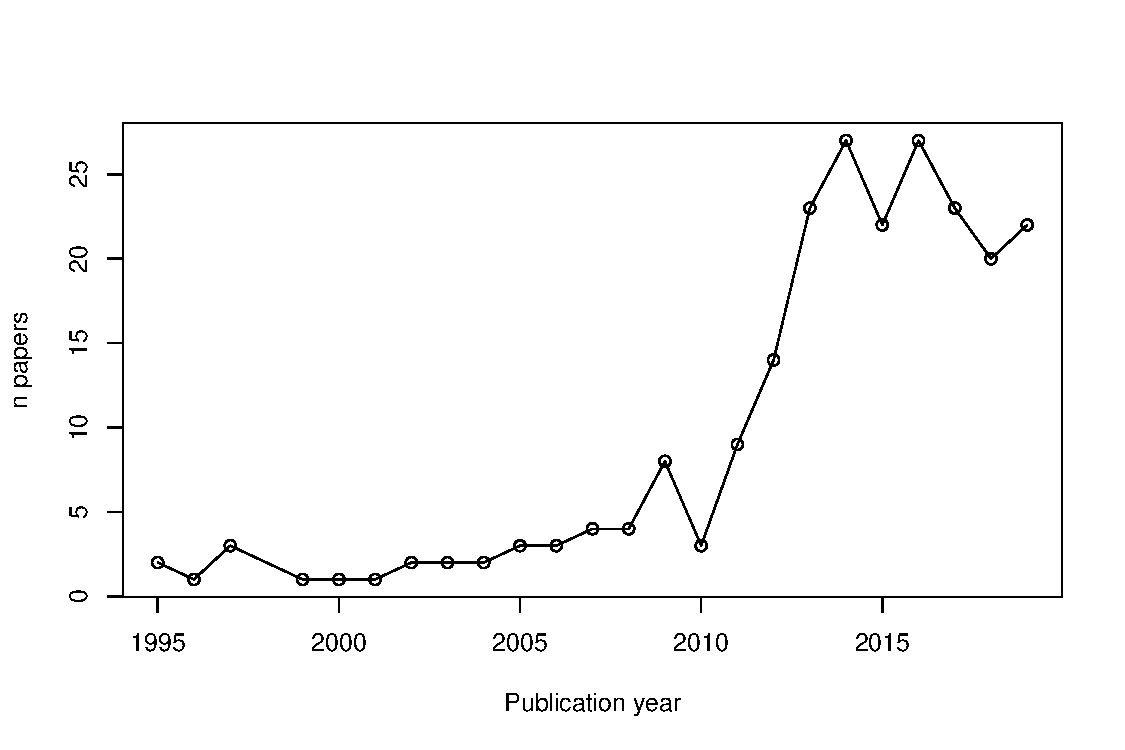
\includegraphics[width=1\textwidth]{..//..//R/graphs/otherdat/papersovertime.pdf}
\caption{Trends in all papers using search terms over time. Of papers from which we could extract data all were published in 2016 or onward.}
  \label{fig:papertrends}
\end{figure}


\newpage 
\section{Model}

\subsection{Dimensional analysis}
\begin{center}
\begin{table}[h!]
\caption{Table of parameter values, their definitions and lightweight version of their dimensions (i.e., not yet deemed `grams' or such).}
\begin{tabular}{ | p{3.0cm} | p{6.0cm} | p{4.0cm} |}
\hline 
Parameter & Definition & Unit \\ \hline 
\end{tabular}
\begin{tabular}{ | p{3.0cm} | p{6.0cm} | p{4.0cm} |}
\(N_{i}\) & seedbank of species \(i\) & seeds \\ \hline
\(s_{i}\) & survival of species \(i\) & unitless \\ \hline
\(\delta\) (peak biomass) & total length of growing season & days\\ \hline
\(B_{i}\) & biomass of species \(i\) & biomass \\ \hline
\(R\) & resource & resource\\ \hline
\(c_{i}\) & conversion of \(R\) uptake to biomass of species \(i\) &  \(\frac{\text{biomass}}{\text{resource}}\) \\ \hline
\(m_{i}\) & maintenance costs of species \(i\) & \(\text{days}^{-1}\) \\ \hline
\(a_{i}\) & uptake increase as \(R\) increases for species \(i\) & \(\text{days}^{-1}\) \\ \hline
\(u_{i}\) & max uptake for species \(i\) & \(\frac{(\text{days})(\text{biomass})}{\text{resource}}\) \\ \hline
\(\phi_{i}\) & converesion of biomass to seedbank for species, includes overwintering of seeds \(i\) & \(\text{biomass}^{-1}\), but conceptually \(\frac{\text{seeds}}{(\text{biomass})(\text{seeds})}\) \\ \hline
\(\epsilon\) & abiotic loss of \(R\) &  \(\text{days}^{-1}\) \\ \hline
\(g_{max,i}\) & max germination of species \(i\) & unitless \\ \hline
\(h_{i}\) &  controls the the rate at which germination declines as \(\tau_{p}\) deviates from optimum for species \(i\)  & \(\text{days}^{-2}\) \\ \hline
\(g_{i}\) & germination fraction & unitless \\ \hline
\(\tau_{p}\) & timing of pulse & days \\ \hline
\(\tau_{i}\) & timing of max germination of species \(i\) & days \\ \hline
\(\alpha_{i}\) & phenological tracking of species \(i\) & unitless \\ \hline
\(\theta_{i}\) & shape of uptake for species \(i\) & unitless\\ \hline
\hline
\(b_{i}\) & seedling biomass of species \(i\) & \(\frac{\text{biomass}}{\text{seeds}}\) \\ \hline
\(f_{i}(R)\) & \(R\) uptake \(f(x)\) for species \(i\) & \(\frac{\text{resource}}{(\text{days})(\text{biomass})}\)\\ \hline
\(d_{i}\) & death rate of species \(i\), used in calculations of lifespan & unitless \\ \hline
\(t\) & between year time (formerly T) & years \\ \hline
\(0\) $\rightarrow$ \(\delta\) & within season time (formerly \(\tau\)) & days \\ \hline
\(b_{0}\) & initial biomass per germinant (seed) & biomass \\ \hline
\(\xi\) & \(\frac{\text{final biomass}}{\text{initial biomass}}\) & unitless \\ \hline
\hline
\end{tabular}
\end{table}
\end{center}

\section{Model runs}


\emph{Analyses}: Ran XX models ...
\end{document}